% $Id$

%\subsection{Design and Implementation Notes}

The VM class provides an additional layer of abstraction on top of the POSIX machine model, making it suitable for HPC applications. There are four key aspects the VM class deals with.

\begin{enumerate}

\item Encapsulation of hardware and operating system details within the concept of Persistent Execution Threads (PETs).

\item Resource management in terms of PETs with a guard against over-subscription.

\item Topological description of the underlying configuration of the compute resources in terms of PETs.

\item Transparent communication API for point-to-point and collective PET-based primitives, hiding the many different communication channels and offering best possible performance.

\end{enumerate}

\begin{center}
\scalebox{0.6}{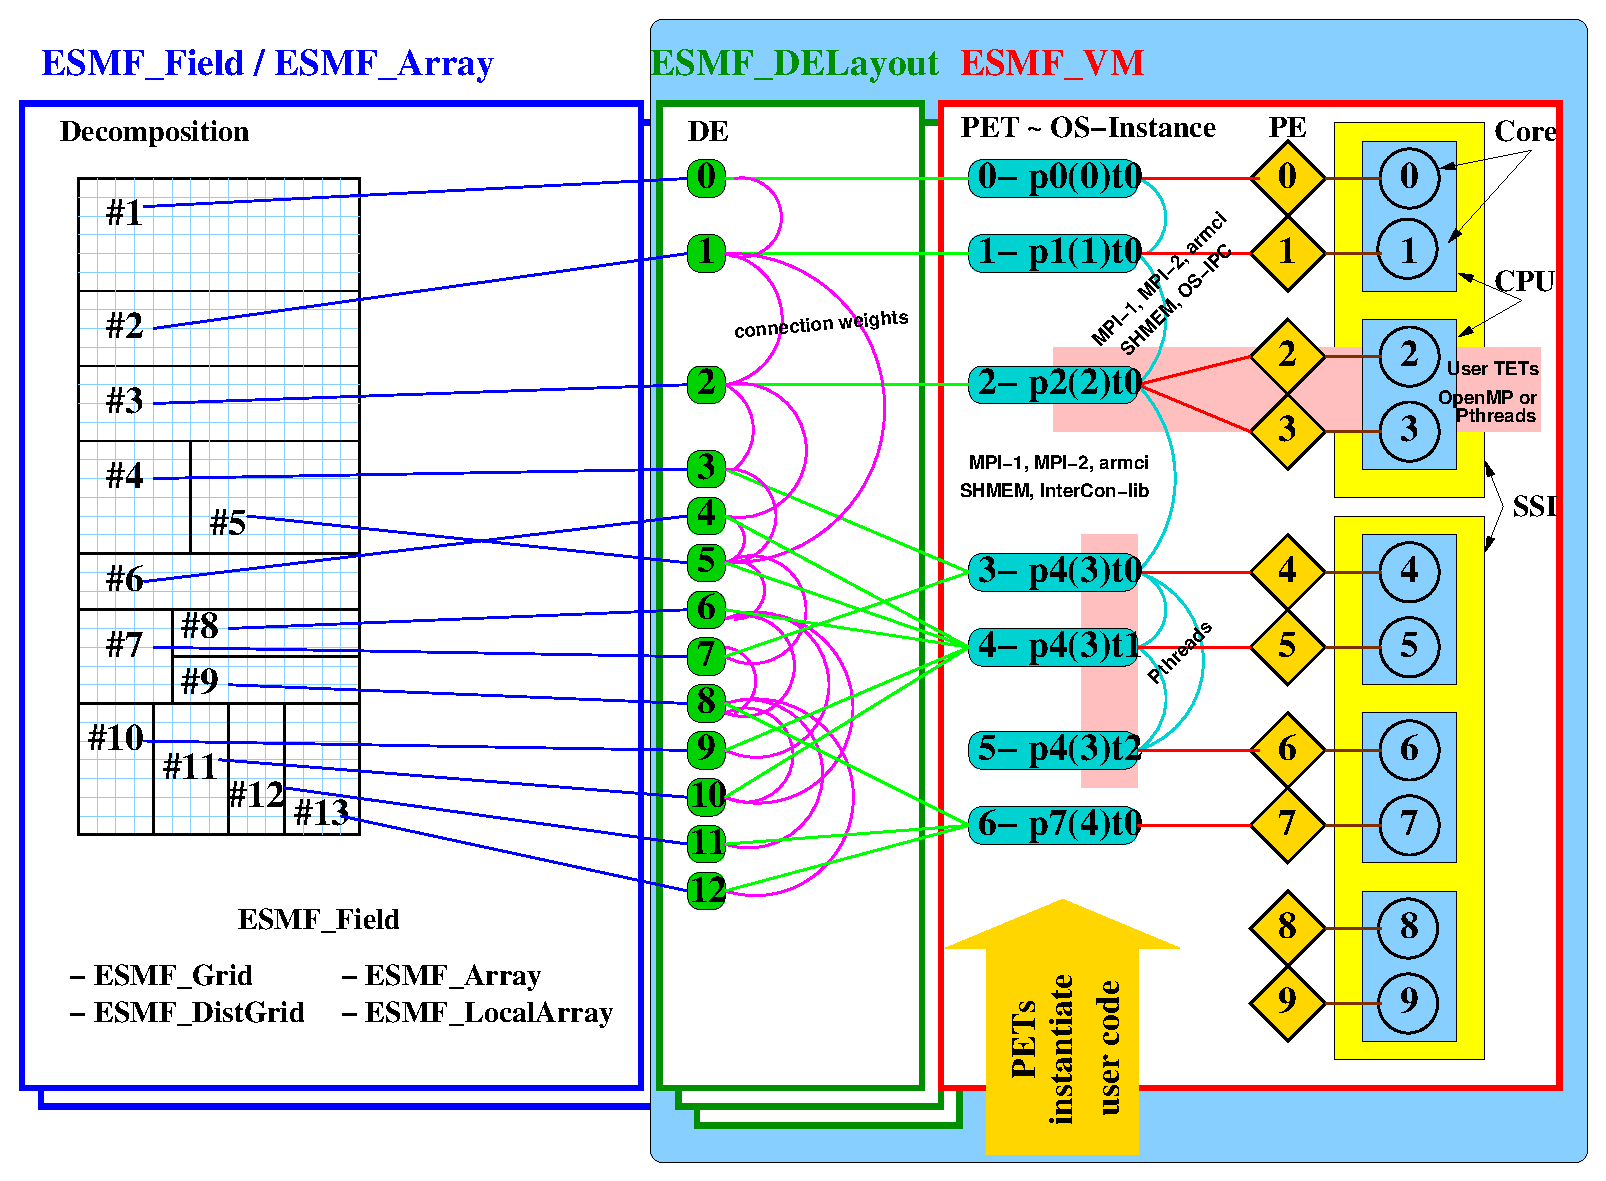
\includegraphics{VM_design}}
\end{center}


{\bf Definition of terms used in the diagram}

\begin{itemize}

\item PE: A processing element (PE) is an alias for the smallest physical processing unit available on a particular hardware platform. In the language of today's microprocessor architecture technology a PE is identical to a core, however, if future microprocessor designs change the smallest physical processing unit the mapping of the PE to actual hardware will change accordingly. Thus the PE layer separates the hardware specific part of the VM from the hardware-independent part. Each PE is labeled with an id number which identifies it uniquely within all of the VM instances of an ESMF application.

\item Core: A Core is the smallest physical processing unit which typically comprises a register set, an integer arithmetic unit, a floating-point unit and various control units. Each Core is labeled with an id number which identifies it uniquely within all of the VM instances of an ESMF application.

\item CPU: The central processing unit (CPU) houses single or multiple cores, providing them with the interface to system memory, interconnects and IO. Typically the CPU provides some level of caching for the instruction and data streams in and out of the Cores. Cores in a multi-core CPU typically share some caches. Each CPU is labeled with an id number which identifies it uniquely within all of the VM instances of an ESMF application.

\item SSI: A single system image (SSI) spans all the CPUs controlled by a single running instance of the operating system. SMP and NUMA are typical multi-CPU SSI architectures. Each SSI is labeled with an id number which identifies it uniquely within all of the VM instances of an ESMF application.

\item TOE: A thread of execution (TOE) executes an instruction sequence. TOE's come in two flavors: PET and TET.

\item PET: A persistent execution thread (PET) executes an instruction sequence on an associated set of data. The PET has a lifetime at least as long as the associated data set. In ESMF the PET is the central concept of abstraction provided by the VM class. The PETs of an VM object are labeled from 0 to N-1 where N is the total number of PETs in the VM object.

\item TET: A transient execution thread (TET) executes an instruction sequence on an associated set of data. A TET's lifetime might be shorter than that of the associated data set.

\item OS-Instance: The OS-Instance of a TOE describes how a particular TOE is instantiated on the OS level. Using POSIX terminology a TOE will run as a single thread within a single- or multi-threaded process.

\item Pthreads: Communication via the POSIX Thread interface.

\item MPI-1, MPI-2: Communication via MPI standards 1 and 2.

\item armci: Communication via the aggregate remote memory copy interface.

\item SHMEM: Communication via the SHMEM interface.

\item OS-IPC: Communication via the operating system's inter process communication interface. Either POSIX IPC or System V IPC.

\item InterCon-lib: Communication via the interconnect's library native interface. An example is the Elan library for Quadrics.

\end{itemize}

The POSIX machine abstraction, while a very powerful concept, needs augmentation when applied to HPC applications. Key elements of the POSIX abstraction are processes, which provide virtually unlimited resources (memory, I/O, sockets, ...) to possibly multiple threads of execution. Similarly POSIX threads create the illusion that there is virtually unlimited processing power available to each POSIX process. While the POSIX abstraction is very suitable for many multi-user/multi-tasking applications that need to share limited physical resources, it does not directly fit the HPC workload where over-subscription of resources is one of the most expensive modes of operation.

ESMF's virtual machine abstraction is based on the POSIX machine model but holds additional information about the available physical processing units in terms of Processing Elements (PEs). A PE is the smallest physical processing unit and encapsulates the hardware details (Cores, CPUs and SSIs).

There is exactly one physical machine layout for each application, and all VM instances have access to this information. The PE is the smallest processing unit which, in today's microprocessor technology, corresponds to a single Core. Cores are arranged in CPUs which in turn are arranged in SSIs. The setup of the physical machine layout is part of the ESMF initialization process.

On top of the PE concept the key abstraction provided by the VM is the PET. All user code is executed by PETs while OS and hardware details are hidden. The VM class contains a number of methods which allow the user to prescribe how the PETs of a desired virtual machine should be instantiated on the OS level and how they should map onto the hardware. This prescription is kept in a private virtual machine plan object which is created at the same time the associated component is being created. Each time component code is entered through one of the component's registered top--level methods (Initialize/Run/Finalize), the virtual machine plan along with a pointer to the respective user function is used to instantiate the user code on the PETs of the associated VM in form of single- or multi-threaded POSIX processes.

The process of starting, entering, exiting and shutting down a VM is very transparent, all spawning and joining of threads is handled by VM methods "behind the scenes". Furthermore, fundamental synchronization and communication primitives are provided on the PET level through a uniform API, hiding details related to the actual instantiation of the participating PETs.

Within a VM object each PE of the physical machine maps to 0 or 1 PETs. Allowing unassigned PEs provides a means to prevent over-subscription between multiple concurrently running virtual machines. Similarly a maximum of one PET per PE prevents over-subscription within a single VM instance. However, over-subscription is possible by subscribing PETs from different virtual machines to the same PE. This type of over-subscription can be desirable for PETs associated with IO work loads expected to be used infrequently and to block often on IO requests.

On the OS level each PET of a VM object is represented by a POSIX thread (Pthread) either belonging to a single-- or multi--threaded process and maps to at least 1 PE of the physical machine, ensuring its execution. Mapping a single PET to multiple PEs provides resources for user--level multi--threading, in which case the user code inquires how many PEs are associated with its PET and if there are multiple PEs available the user code can spawn an equal number of threads (e.g. OpenMP) without risking over-subscription. Typically these user spawned threads are short-lived and used for fine-grained parallelization in form of TETs. All PEs mapped against a single PET must be part of a unique SSI in order to allow user--level multi--threading!

In addition to discovering the physical machine the ESMF initialization process sets up the default global virtual machine. This VM object, which is the ultimate parent of all VMs created during the course of execution, contains as many PETs as there are PEs in the physical machine. All of its PETs are instantiated in form of single-threaded MPI processes and a 1:1 mapping of PETs to PEs is used for the default global VM.

The VM design and implementation is based on the POSIX process and thread model as well as the MPI-1.2 standard. As a consequence of the latter standard the number of processes is static during the course of execution and is determined at start-up. The VM implementation further requires that the user starts up the ESMF application with as many MPI processes as there are PEs in the available physical machine using the platform dependent mechanism to ensure proper process placement. 

All MPI processes participating in a VM are grouped together by means of an MPI\_Group object and their context is defined via an MPI\_Comm object (MPI intra-communicator). The PET local process id within each virtual machine is equal to the MPI\_Comm\_rank in the local MPI\_Comm context whereas the PET process id is equal to the MPI\_Comm\_rank in MPI\_COMM\_WORLD. The PET process id is used within the VM methods to determine the virtual memory space a PET is operating in. 

In order to provide a migration path for legacy MPI-applications the VM offers accessor functions to its MPI\_Comm object. Once obtained this object may be used in explicit user-code MPI calls within the same context.


